\documentclass{standalone}
\usepackage{tikz}
\usepackage{ctex,siunitx}
\setCJKmainfont{Noto Serif CJK SC}
\usepackage{tkz-euclide}
\usepackage{amsmath}
\usetikzlibrary{patterns, calc}
\usetikzlibrary {decorations.pathmorphing, decorations.pathreplacing, decorations.shapes,}
\begin{document}
\small
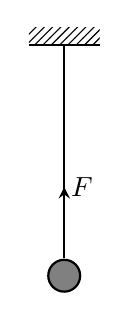
\begin{tikzpicture}[>=stealth, thick,scale=0.9]
  % \useasboundingbox(-1,-0.75)rectangle(3.7,1.4);
  \fill [pattern = north east lines] (0,0) rectangle (1,.25);
  \draw(0,0)--(1,0);
  \draw(.5,0)--(.5,-3);
  \draw [fill=black!50] (.5,-3.25) circle (.225);
  \draw[->](.5,-3)--(.5,-2);
  \node at (.75,-2){$F$};
  \end{tikzpicture}
\end{document}